\documentclass[11pt]{article}
\usepackage[dvipsnames]{xcolor}
\usepackage[T1]{fontenc}
\usepackage{mathtools}
\usepackage[french]{babel}
\usepackage{amsmath,amssymb,amsthm}
\usepackage{framed}
\usepackage{lmodern}
\usepackage{utils}
\usepackage{pdfpages}
\usepackage{irif}
\usepackage{listings}
\usepackage{listingsutf8}

\definecolor{codegreen}{rgb}{0,0.6,0}
\definecolor{codegray}{rgb}{0.5,0.5,0.5}
\definecolor{codepurple}{rgb}{0.58,0,0.82}
\definecolor{backcolour}{rgb}{0.96,0.96,0.95}

\lstdefinestyle{mystyle}{
    backgroundcolor=\color{backcolour},
    commentstyle=\color{codegreen},
    keywordstyle=\color{magenta},
    numberstyle=\tiny\color{codegray},
    stringstyle=\color{codepurple},
    basicstyle=\ttfamily\footnotesize,
    breakatwhitespace=false,
    breaklines=true,
    captionpos=b,
    keepspaces=true,
    numbers=left,
    numbersep=5pt,
    showspaces=false,
    showstringspaces=false,
    showtabs=false,
	extendedchars=true,
    tabsize=4,
	basicstyle=\ttfamily,
  	mathescape,
	inputencoding=utf8/latin1,
	literate=%
		{é}{{\'e}}{1}%
		{è}{{\`e}}{1}%
		{à}{{\`a}}{1}%
		{ç}{{\c{c}}}{1}%
		{œ}{{\oe}}{1}%
		{ù}{{\`u}}{1}%
		{É}{{\'E}}{1}%
		{È}{{\`E}}{1}%
		{À}{{\`A}}{1}%
		{Ç}{{\c{C}}}{1}%
		{Œ}{{\OE}}{1}%
		{Ê}{{\^E}}{1}%
		{ê}{{\^e}}{1}%
		{î}{{\^i}}{1}%
		{ô}{{\^o}}{1}%
		{û}{{\^u}}{1}%
		{ë}{{\¨{e}}}1
		{û}{{\^{u}}}1
		{â}{{\^{a}}}1
		{Â}{{\^{A}}}1
		{Î}{{\^{I}}}1
}

\lstset{style=mystyle}

\begin{document}
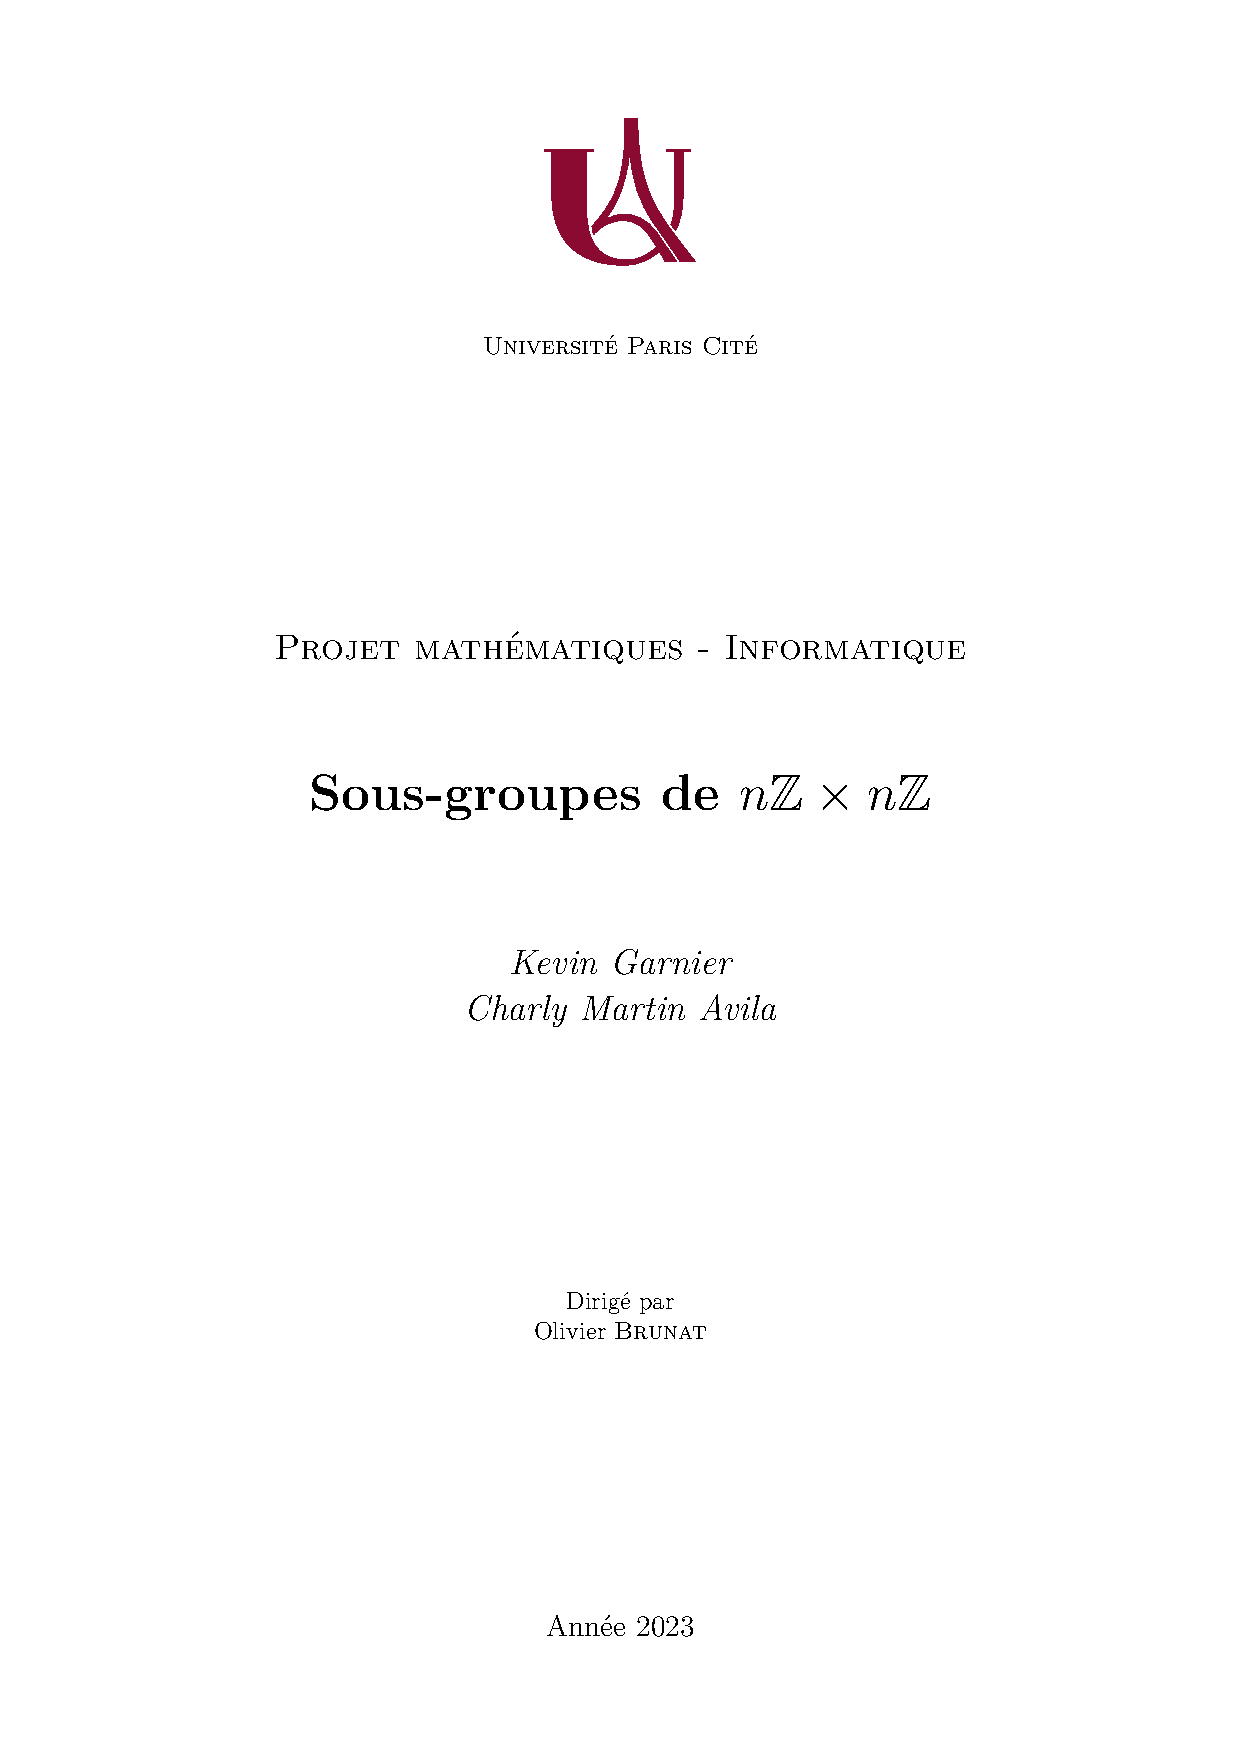
\includepdf{title.pdf}
\tableofcontents
\newpage

\section{Introduction}
Il est très facile de décrire tous les sous-groupes d'un groupe cyclique
d'ordre $n$ : il y en a exactement un par diviseur positif de $n$.
Pourtant, étonnamment, décrire tous les sous-groupes d'un groupe abélien
est en général un problème difficile.\\
Dans ce projet, nous nous se proposons de considérer cette question pour le groupe $\ZZ$.

D'un point de vue théorique, nous mettrons en avant la générations et la caractérisations de \\
sous-groupes grâce aux vecteurs colonne des matrices à coefficients entier et en particulier aux formes
normales de Hermite. Nous montrerons aussi une formule permettant de les compter.

D'un point de vue pratique, nous créerons un programme \textsc{OCaml} capable de générer les\\
sous-groupes de $\ZZ$ ainsi que leur treillis à partir d'un entier donné en paramètres.
\section{Quelques simplifications du problème}
\subsection{Décomposition de $n$ en éléments irréductibles}

Nous pouvons tout d'abord simplifier le problème aux cas où $n = p^m$ avec $p$ un nombre premier
et $m \in \N$. En effet la proposition suivante nous garantie que le résultat est isomorphe
\begin{proposition}
	Soit $n = \prod\limits_i^k p_i^{\alpha_i}$, avec $p_i$ des nombres premiers, alors
	$$(\ZZ) \isom \prod_i^k(\Z/p_i^{\alpha_i}\Z)^2$$
\end{proposition}

\begin{proof}
	Soit $n = \prod\limits_i^k p_i^{\alpha_i}$. Par le théorème des restes chinois, on a
	$$ \ZnZ \isom (\Z/p_i^{\alpha_i}\Z) \x \cdots \x (\Z/p_i^{\alpha_i}\Z)$$
	En particulier,
	\begin{equation*}
		\begin{split}
			\ZZ & \isom
			(\Z/p_i^{\alpha_i}\Z) \x \cdots \x (\Z/p_i^{\alpha_i}\Z) \x (\Z/p_i^{\alpha_i}\Z) \x \cdots \x (\Z/p_i^{\alpha_i}\Z)\\
			& \isom (\Z/p_i^{\alpha_i}\Z)^2 \x \cdots \x (\Z/p_i^{\alpha_i}\Z)^2
		\end{split}
	\end{equation*}
\end{proof}

En pratique, pour décomposer en entier en facteurs irréductibles, nous avons utilisé la procédure de
\textsc{$\rho$-Pollard} pour obtenir un diviseur de $n$:
\begin{lstlisting}
fonction rho_pollard P n x y k i d
    Si d <> 1:
        Retourne d
    Sinon:
        x = P(x) mod n
        d = pgcd(|y - x|, n)
        Si i = k:
            Alors Retourne rho_pollard loop P n x x 2k (i + 1) d
        Sinon Retourne rho_pollard P n x y k (i + 1) d
\end{lstlisting}
Puis nous répétons la procédure jusqu'à que les diviseurs soient premier.\\
En triant et en regroupant les nombres premier, nous obtenons donc les différents $p^{\alpha_i}_i$.\\
Dans notre implémentation, $P(X) = X^2 - 1$ et $n$ n'est pas premier.
%TODO : Ajout algo test primarite ?

\newpage
\subsection{Simplification des sous-groupes}

\begin{proposition}
	$$\Z^2/n\Z \x n\Z \isom \ZZ $$
\end{proposition}
\begin{proof}
	Soit \app{\varphi}{\Z^2}{\ZZ}{(a,b)}{(\bar a, \bar b)}
	$\varphi$ est surjective par définition de la classe d'équivalence de a et b.
	Montrons que $\ker \varphi = n\Z \x n\Z$.

	\begin{equation*}
		\begin{split}
			&(a,b) \in \ker \varphi \\
			&\text{ssi } \varphi(a,b) = (\bar 0, \bar 0)\\
			&\text{ssi } (\bar a, \bar b) = (\bar 0, \bar 0)\\
			&\text{ssi } \bar a = \bar 0 \text{ et } \bar b = \bar 0\\
			&\text{ssi } a \in n\Z \text{ et } b \in n\Z\\
			&\text{ssi } (a,b) \in  n\Z \x n\Z
		\end{split}
	\end{equation*}
	Ainsi par le premier théorème d'isomorphisme, on a
	$$\Z^2/n\Z \x n\Z \isom \ZZ $$
\end{proof}
Ainsi le problème se résout à trouver les sous-groupes $G$ de $\Z^2$ tels que
$H = \matsqr{a}{0}{b}{c}$\\
et
$n\Z \x n\Z \subseteq G = \gen{\vectcolsqr{\bar a}{\bar b}, \vectcolsqr{0}{\bar c}}$


\section{Matrices à coefficients entier et forme normales de Hermite}
Nous avons vu dans la section précédente qu'il était possible de caractériser les sous-groupe de
$\ZZ$ par une matrice $H = \matsqr{a}{0}{b}{c}$. Cependant, ces matrices ne sont pas uniques. C'est
pourquoi, nous allons utiliser les formes normales d'Hermite.
Énonçons d'abord quelques propriété sur les matrices à coefficients entier.
%problème section précédente, il existe un nombre important de matrice similaire i.e qui
%engendre le même sous groupe
\subsection{Matrices à coefficients entier}
\begin{proposition}
	Soient $A \in \M_{m,n}(\Z)$ et $Q \in \GL_n(\Z)$, alors
	$$\im AQ = \im A$$
\end{proposition}
\begin{proof}
	Soit $y \in \im AQ$, il existe $x \in \Z^n$ tel que $y = AQx$. Or,
	\begin{align*}
		         & y = AQx     \\
		\implies & y = A(Qx)   \\
		\implies & y \in \im A
	\end{align*}
	Donc $\im AQ \subseteq \im A$.\\
	Soit $y \in \im A$. Il existe $x \in \Z^n$ tel que $y = Ax$.\\
	Cherchons $z \in \Z^n$ tel que $y = Ax = AQz$
	\begin{align*}
		         & Ax = AQz                                     \\
		\implies & A(x) = A(Qz)                                 \\
		\implies & x = Qz                                       \\
		\implies & \inv Q x = z \text{ (car $B \in \GL_n(\Z)$)}
	\end{align*}
	Donc il existe bien un $z \in \Z^n$ tel que $ABz = y$. Donc $y \in \im AQ$.\\
	D'où $\im AQ = \im A$

\end{proof}
\subsection{Formes normales de Hermite}
Nous allons désormais énoncer quelques propriétés utiles sur les formes normales de Hermite.
\begin{definition}
	Soit $A \in \M_{m,n}(\Z)$. Alors il existe une unique matrice échelonnée
	réduite suivant les colonnes $H \in \M_{m,n}(\Z)$ telle qu'il existe $Q \in \GL_n(\Z)$
	avec $H = AQ$. La matrice $H$ s'appelle la forme normale de Hermite de A.
\end{definition}

\begin{proof}


	Nous supposerons l'unicité admise, l'algorithme suivant nous montre son existence.

	\begin{lstlisting}
Fonction hermite $A$:
	Pour chaque $i$ de 1 à $n$ :
		trier la ligne de la colonne $i$ à la colonne $n$
		Pour chaque $j$ de $i$ à $m$:
			Si $a_{ij} < 0$, réaliser l'opération($C_j \longleftarrow -C_j$)
        	$k$,$r$ = div_euclide($a_{ij}$, $a_{ii}$)
            réaliser l'operation $C_j \longleftarrow C_j - kC_i$
		Si la ligne n'est pas réduite :
			recommencer la boucle

	Retourner A
\end{lstlisting}

	\begin{lstlisting}
	let rec hermite_loop_line (mat, t) i j m =
  match resolve_null (mat, t) i with
  | None -> (mat, t)
  | Some mt ->
      if j >= m then
        if is_reduced mt i then reduce_left mt i
        else hermite_loop_line (permut_min mt i) i i m
      else if i == j then
        if mat.(i).(j) < 0 then hermite_loop_line (change_sign mt i) i (j + 1) m
        else hermite_loop_line mt i (j + 1) m
      else hermite_loop_line (reduce mt i j i) i (j + 1) m

let rec hermite_loop (mat, t) i =
  let n, m = size mat in
  if i >= n || i >= m then (mat, t)
  else hermite_loop (hermite_loop_line (mat, t) i 0 m) (i + 1)
\end{lstlisting}

\begin{lstlisting}
Fonction hermite $A$:
	Pour chaque $i$ allant de 1 à $m$ :
		Pour chaque $j$ allant de  
		Si $\forall i < j <= m, a_{ij} = 0$:
			Continuer boucle
		Permuter $C_j$ contenant $a_{ij} = \min(\mset{a_{ij}}{i <= j <= n a_{ij} \ne 0})$ avec $C_i$
\end{lstlisting}

	Montrons la terminaison de l'algorithme.\\
	À chaque tour de boucle $i$, nous réalisons une réduction de la ligne grâce à la division
	euclidienne.\\
	Et $\forall j, a^{(n)}_{ij} < a^{(n + 1)}_{ij}$ où $a^{(k)_{ij}}$ est la valeur de $a_{ij}$
	au $k^e$ tour de boucle. Donc il existe un rang $N$, où la ligne sera réduite au maximum.
	Ce qui nous permet de traiter les lignes restantes. Donc l'algorithme termine bien.\\
	Montrons sa correction.
	À chaque tour de boucle $i$, si la ligne n'est pas réduite,
	alors on continue de la réduire avant de la passer à la suivante. Cela nous assure donc que le lignes sont bien réduites.
	Ainsi à la fin des boucles, les lignes sont bien réduites.



\end{proof}

% preuve existence ?
% algo forme hermite
% preuve AX = C solution ssi on peut annuler C ?

\section {Génération et énumération des sous-groupes}
\subsection{Génération des sous-groupes}
%preuve sur la bonne forme de forme normale de Hermite
\subsection{Énumération des sous-groupes}
%preuve sur le calcul du nombre de sous-groupe

\section{Génération du treillis}
%preuve H C H' <=> Hermite(H'|H) = H'
%Algorithme génération du treillis
%Choix de .dot et graphivz

\section{Quelques résultats}
\subsection{Pour n = 2}
%pour n = 2
\subsection{Pour n = 4}
% pour n = 4
\subsection{Pour n = 20}
% pour n = 20

%nombre de sous-groupes + treillis .dot

\section{Références}
%livre d'algo
%poly du prof

\end{document}
